\chapter{Product manual}

\section{Project setup}
This section is meant for the xmd software maintainer or researcher.

\begin{itemize}
\item install Qt 5.4.0
\item install Qt Installer Framework 1.5.0
\item install Google test
\item install Git
\item install Latex tool
\item clone xMAS repository
\end{itemize}

Once the project is setup, open $''.../xmas/src/main.pro''$ with Qt Creator.
Set xmdmain as default and build the Qt project.

\section{Installer}
This section is meant for xmd end users who want to design and verify xMAS models.

Go to the xMAS webpage and download the appropriate installer. For example,
choose $''xmd-windows-x86-1.0.0.exe''$ for a 32bit MS Windows platform. After
the download was successful start it and follow the install procedure.
If the installation is finished xmd can be started via the desktop icon or the startmenu.

\begin{tcolorbox}[colback=white]
\textbf{
At the moment there is only a Windows installer available and can be found in
the xmas repository in the ``installers'' map.
}
\end{tcolorbox}

\section{xMAS model design}
This section first starts with explaining the main parts of the user interface,
secondly how to set it up and finally how to create and save an xMAS model.

\subsection{Main window}
Figure~\ref{fig:mainwindow} is the main window of the designer application. On
top there is the xMAS toolbar while in the center it has a single page canvas
that can be setup. A tabbed console can be found at the bottom, the first tab
selects the designer console. Every verification tool loaded as plug-in get its
own console which can be selected via a tab named as the plug-in.

\begin{figure}[here]
\begin{center}	
	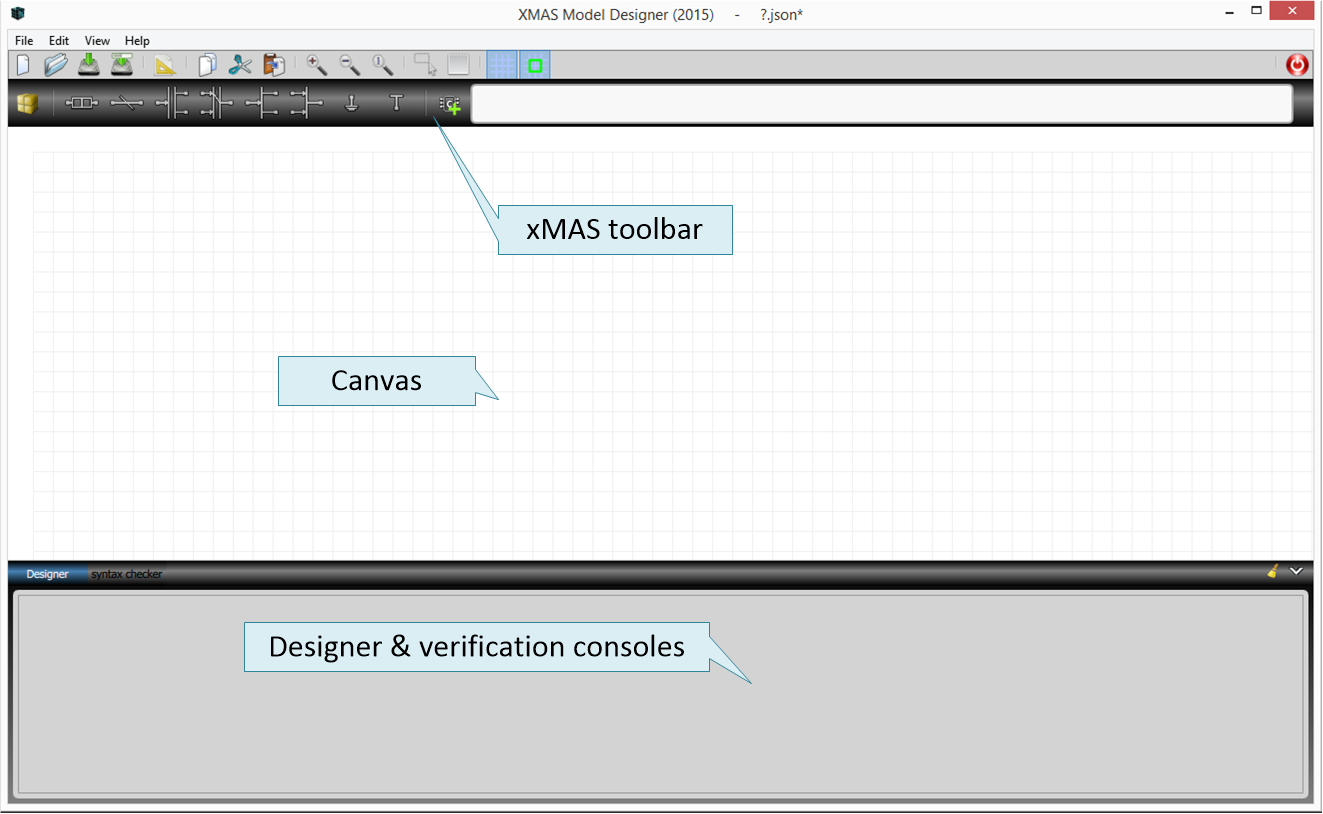
\includegraphics[width=.70\linewidth]{pictures/xmd-empty}
	\caption{Main application window}
	\label{fig:mainwindow}
\end{center}
\end{figure}

\subsection{xMAS tool bar}
The xMAS toolbar (figure~\ref{fig:xmas-toolbar}) holds the items that can be
used to create a model. The packet setup button opens a dialog to set up the
model packet. The xMAS language has only eight primitive components and can be
found next to the packet button. 

\begin{figure}[here]
\begin{center}	
	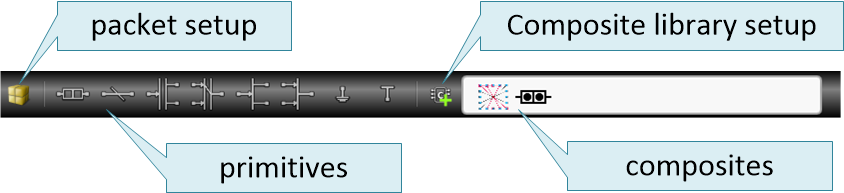
\includegraphics[width=.70\linewidth]{pictures/xmas-toolbar}
	\caption{xMAS toolbar}
	\label{fig:xmas-toolbar}
\end{center}
\end{figure}

Composite components can be found at the right part of this toolbar. Primitive
and composite components can be placed on the canvas by dragging. The area
holding the available composites is called the library which is a horizontal
flickable list. The button at the left side of this list opens a dialog to add a
composite. To remove a composite simply right click the composite and select
remove. Notice that a composite can only be removed if it is not used.


\subsection{Canvas}
The canvas is build as a flickable single page. The actual view port of this page
can be changed by drag or swipe it. The size of the canvas page can be changed
in the model setup dialog and is saved with the model. The minimum size is 500
by 500 while the maximum size is 5000 by 5000. This means that the largest
models can directly hold 500 normal scaled primitive components or 2000 if small
scaled.

\paragraph{With grid and snap} canvas items can be easily aligned. The main
toolbar has two toggle buttons, one to show or hide the canvas grid and one to
set the grid snap ``on'' or ``off''.

\begin{figure}[here]
\begin{center}	
	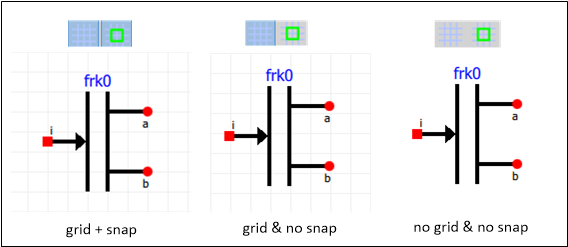
\includegraphics[width=.70\linewidth]{pictures/canvas-grid}
	\caption{canvas grid \& snap options}
	\label{fig:canvas-grid}
\end{center}
\end{figure}





\subsection{Console}



\section{xMAS model verification}
\begin{tcolorbox}[colback=white]
\textbf{
In the current project, only the syntax checker is adopted with a plug-in
interface and can be used via the GUI.
}
\end{tcolorbox}



\section{Remarks}

\begin{tcolorbox}[colback=yellow!30]
 verwijzing naar appendix voor feature,fix en bug list
\end{tcolorbox}



%%\newpage

